\documentclass[journal]{IEEEtran}
\usepackage{blindtext}
\usepackage{graphicx}
\usepackage{subfig}
\usepackage[english]{babel}
\usepackage{pinyin}
\usepackage{natbib}
\usepackage{notoccite}
\usepackage{amssymb}
\usepackage{textcomp}
\usepackage{floatrow}
\usepackage{amsmath}
%
\begin{document}
%
% paper title
\title{Real-Time Activity Classification by Match Filtering using Body-Worn Accelerometers}
%
\author{Craig~Euler, Bryan~Juarez, Melissa~Flores, C.T.~Lin}
%
\maketitle
%
\begin{abstract}
Body worn sensors have been used in the market for many years now.
Many of which are used for activity monitoring or fitness.
In this paper, we make use of a matched-filtering algorithm for activity classification with data obtained from three-axis accelerometers worn by the user.
We show real-time processing capability on the MSP432 microcontroller hardware.
We achieve invariance to sensor orientation with dimensionality reduction.
We make use of an instance-based learning algorithm to train the device to learn the individual's motion patterns and store that information as activity filters for our matched filter.
We improve computational efficiency with dimensionality reduction, decimation in time, and pre-processing of our references post training for use in the matched-filter.
An assessment of our processing time is provided with runtime experiments on the MSP432 microcontroller which shows feasibility of real-time processing capability.
\end{abstract}
%
\section{Introduction}
Various methods for activity classification using body-worn sensors exist.
Custom decision tree, automatically generated decision tree, and artificial neural networks \cite{parkka_ermes_korpipaa_mantyjarvi_peltola_korhonen_2006} have been explored as well as other frequency based classification methods \cite{sharma_purwar_lee_lee_chung_2008}.
In this paper, we make use of a matched-filter method to identify an individual\textquotesingle s activity for the purpose of real-time processing.
The matched-filter method with use of thresholding and comparing the correlations of various filters is a simple method to use and have been studied in the past \cite{giannakis_tsatsanis_1990}.
Many of the algorithms and software structure were tailored to computational efficiency to accommodate the resource limitations on the MSP432 microprocessor.
Having an a priori knowledge of the activity the individual is performing is useful for many current fitness algorithms.

The algorithms described in this paper are broken into two main modules: Training the device to identify the user\textquotesingle s activity, and the real-time activity classification itself.

The training module does not need to be performed in real time.
This algorithm is the most demanding on computational resources and is only ran when training or re-training the unit to identify the user\textquotesingle s activity, so this can be performed on an external device such as a smart phone or tablet.
The purpose of the training module is to create the reference signal to be used on the microcontroller for real-time processing.

The second module is the real-time activity classification on the unit.
This module reads in the reference(s) stored on the unit to be used as templates that the matched-filter will use for determining the individual\textquotesingle s activity.
Both of these modules use the same principles and hence the same algorithm kernels.
%
\section{The Algorithms}
%
\subsection{Activity Classification Method}
The matched-filter method is commonly used for extracting a signal out of noisy data.
We use this method for identifying a user\textquotesingle s activity from data generated by body-worn accelerometers.
Because the matched-filter method requires use of an existing reference template to identify the desired signal, we must develop our template from a training set.
We will discuss how we develop our set of templates for use in our matched-filter.

The matched filter is based on the cross correlation of the data $\textbf{y} = \{y\}_{k=0}^{N-1}$ with the reference signal $\textbf{x} = \{x\}_{k=0}^{M-1}$.
The cross correlation of $\textbf{x}$ with $\textbf{y}$ is defined as:
%
\begin{equation} \label{cross_correlation_eq}
(\textbf{x} \star \textbf{y}) = \left \{\sum_{i=0}^{M}x_{i} y_{i+k} \right \}_{k=0}^{N-M-1}
\end{equation}
%
which is simply a moving dot product.
We can then normalize \eqref{cross_correlation_eq} by the following:
%
\begin{equation} \label{norm_cross_correlation_eq}
\widehat{(\textbf{x} \star \textbf{y})}_k = \frac{(\textbf{x} \star \textbf{y})_k}{||\textbf{x}|| \ || \widetilde{\textbf{y}}_k || }, \quad k = 0,1,...,N-M-1
\end{equation}
%
where $|| \cdot ||$ is the usual $\ell_2$ norm and $\widetilde{\textbf{y}}_k = \{y_p\}_{p=k}^{M+k-1}$.
\eqref{norm_cross_correlation_eq} is now bounded by $[-1,1]$ and has any bias toward high energy removed.
We improve our computational efficiency by applying the convolution theorem to \eqref{cross_correlation_eq} and replacing it with:
%
\begin{equation} \label{conv_theorem}
(\textbf{x} \star \textbf{y}) = FFT^{-1}(FFT(\textbf{x}') FFT(\textbf{y})^*)
\end{equation}
%
Where $\textbf{x}'$ is $\textbf{x}$ that has been zero padded to the length of $\textbf{y}$ with the added restriction that the length of $\textbf{x}$ is no more than the length of $\textbf{y}$ and $FFT$ is the Fast Fourier Transform algorithm.
We are most interested where our reference $\textbf{x}$ best matches our data $\textbf{y}$.
We use the resulting max correlation to define our metric for  our matched-filter output as:
%
\begin{equation} \label{matched_filter_eq}
MF_{\textbf{x}}(\textbf{y}) := \underset{k \in [0, M-N)}{max} \left \{\widehat{(\textbf{x} \star \textbf{y})}_k \right \}
\end{equation}
%
If \eqref{matched_filter_eq} passes a threshold, the corresponding signal is a match.
%
\subsection{Dimensionality Reduction}
We manage to reduce our computational resources and remove our dependence on sensor orientation at the same time through a process of dimensionality reduction with principal component analysis (PCA) \cite{bishop_2006}.
We assume that over a short period of time, a user\textquotesingle s limb movement is constrained mostly to a two-dimensional plane.
By identifying this plane of motion, we then project the acceleration data onto this plane and re-define our new axis accordingly.

If we let $\textbf{a} = \{a_i\}_{i=0}^{N}$ represent our demeaned acceleration data over a specified time window in three dimensions then the covariance matrix of our acceleration data is represented by the real-symmetric $3 \times 3$ matrix $Q = \textbf{a} \textbf{a}^T$.
The resulting unit length column eigenvectors of $Q$ are $V = (\textbf{v}^1,\textbf{v}^2,\textbf{v}^3)$ with their respective eigenvalues $\lambda^1 \geq \lambda^2 \geq \lambda^3$ of this matrix are orthonormal and point in the directions where the data varies most in descending order for each orthogonal direction.
% \ref{bishop_2006}
\begin{equation} \label{project_eq}
   \textbf{a}' = V^T \textbf{a}
\end{equation}
%
We now represent our acceleration data as $\textbf{a}'$ after projecting our acceleration data $\textbf{a}$ onto our rotated axis $V$ by \eqref{project_eq}. If the data is mostly dominate in the two primary dimensions, i.e. $\lambda^3 << \lambda^2$, then it is safe to assume that
%
\begin{equation} \label{magnitude_eq}
||(a^1,a^2,a^3)||^2 = ||(a'^1,a'^2,a'^3)||^2 \sim = (a'^1)^2 + (a'^2)^2
\end{equation}
$ \forall a \in \textbf{a}. $ \\
%
Equality comes from the orthonormality of $V$. The margin of error in the approximation is not important since we are only interested in processing in the two dimensions.
By now we have preserved as much information that is contained in our acceleration data as possible while also reducing our dimension from three to two.
By projecting our data onto the plain defined by the two most dominant eigen vectors, we effectively reduce our representation of our data to two dimensions.

To compute the matched-filter output for two dimensions, we generalize \eqref{matched_filter_eq} by augmenting our reference and data with both dimensions appropriately for normalization and adding together the cross correlations as:
%
\begin{equation} \label{cross_correlation_eq_2}
\widehat{(\textbf{x}^{1,2} \star \textbf{y}^{1,2})}_k = \frac{(\textbf{x}^1 \star \textbf{y}^1)_k + (\textbf{x}^2 \star \textbf{y}^2)_k}{||[ \textbf{x}^1, \textbf{x}^2 ]|| \ || [ \widetilde{\textbf{y}}_k^1, \widetilde{\textbf{y}}_k^2 ] || },
\end{equation}
%
for $ k = 0,1,...,N-M-1 $. \\
%
\begin{equation} \label{matched_filter_eq_2}
MF_{\textbf{x}}^2(\textbf{y}) := \underset{k \in [0, M-N)}{max} \left \{\widehat{(\textbf{x}^{1,2} \star \textbf{y}^{1,2})}_k \right \}
\end{equation}
%
This works because both dimensions are always in phase with each other for any given activity and therefore the match will happen in sync.
%
\subsection{Decimation}
Decimation is the first step applied to our data before any additional processing takes place.
Decimation is a process of reducing the sampling rate of a signal.
The process consists of filtering to mitigate any possible aliasing distortion effects followed by a downsampling.
There is a trade off between performance and throughput when we decimate our signal, therefore, we use decimation solely for the purpose of reducing our processing cost.

For our application, we use a triangle filter prior to downsampling. This is achieved by convolving our data with the following weights:
%
\begin{equation} \label{triangle_filter_weights}
w_k^D =
\begin{cases}
  \frac{k+1}{D^2}, & \text{if }\ 0 \leq k < D \\
  \frac{2D - (k + 1)}{D^2}, & \text{if } D \leq k < 2D - 1 \\
  0, & \text{otherwise}
\end{cases}
\end{equation}
%
For a decimation value of $D$. Then the data is downsampled by $D$. This results in:
%
\begin{equation} \label{decimated_signal}
s_k^1 = \sum_{p=0}^{2N-1} w_{p+N(1-k)}^N s_{kN - (p+1)}^0 ?
\end{equation}
%
where $\{s_k^1\}_{k=0}^{M/D}$? is the decimated signal of $\{s_k^0\}_{k=0}^M$?.
\subsection{Training the Module}
We are able to identify an individual\textquotesingle s activity by matching the signal to a reference template.
For our application, we develop a reference signature for our matched filter directly from the person\textquotesingle s motion signature.
We do this by having the individual perform the specific activity over a specified amount of time and select the sub-interval of time that we find best represents the user's motion signature.
For a given activity, we attempt to find the representative periodic signal $s$ of our individual’s activity to be our template for our matched-filter.

If $\textbf{t} = \{t_k\}_{k=0}^{N_t}$ is our training set over $N_t$ data points, we define a collection of subsets $X$ of $\textbf{t}$:
%
\begin{equation} \label{X_subsets_of_training_eq}
X := \left \{ \{t_k\}_{k=p}^{p+M-1} | p=mI \right \}
\end{equation}
%
and $Y$ of $\textbf{t}$:
%
\begin{equation} \label{Y_subsets_of_training_eq}
Y := \left \{ \{t_k\}_{k=p}^{p+N-1} | p=nI \right \}
\end{equation}
%
where $M \leq N$, $I$ is a positive, fixed integer, and $(n,m) \in \mathbb{Z}^2$ where $(m,n)$ vary such that $0 \leq (m,n)I$ and $(m,n)I + (M,N) - 1 \leq N_t$. Then we can determine the representative signal $\textbf{s} \in X$ for our activity that satisfies the condition:
%
\begin{equation} \label{s_condition}
\sum_{y \in Y}MF^2_{\textbf{s}}(\textbf{y}) \geq \sum_{y \in Y}MF^2_{\textbf{x}}(\textbf{y}) \quad \forall \textbf{x} \in X
\end{equation}

We chose this method for its simplicity and robustness against outliers in our training set. We anticipate that the user will have idle motion at the start and end of their training duration when they activate the training mode and with possible disruptions during the process.
%
\section{Results}
%
\subsection{Algorithm Performance}
%
The Kinetisense sensor was used for the algorithm performance analysis in this paper.
This unit has a three-axis accelerometer with an acceleration range of -5g to +5g and a sampling rate of 128Hz.
Samples of walking, jogging, and bicycling have been recorded with this unit attached to the ankle of the user.
A separate instance of walking data has been used specifically for training the classifier.
%
\begin{figure}[!ht]
  %\captionsetup[subfigure]{labelformat=empty}
  \centering
  \subfloat[\label{fig:frac_walking_jogging}]{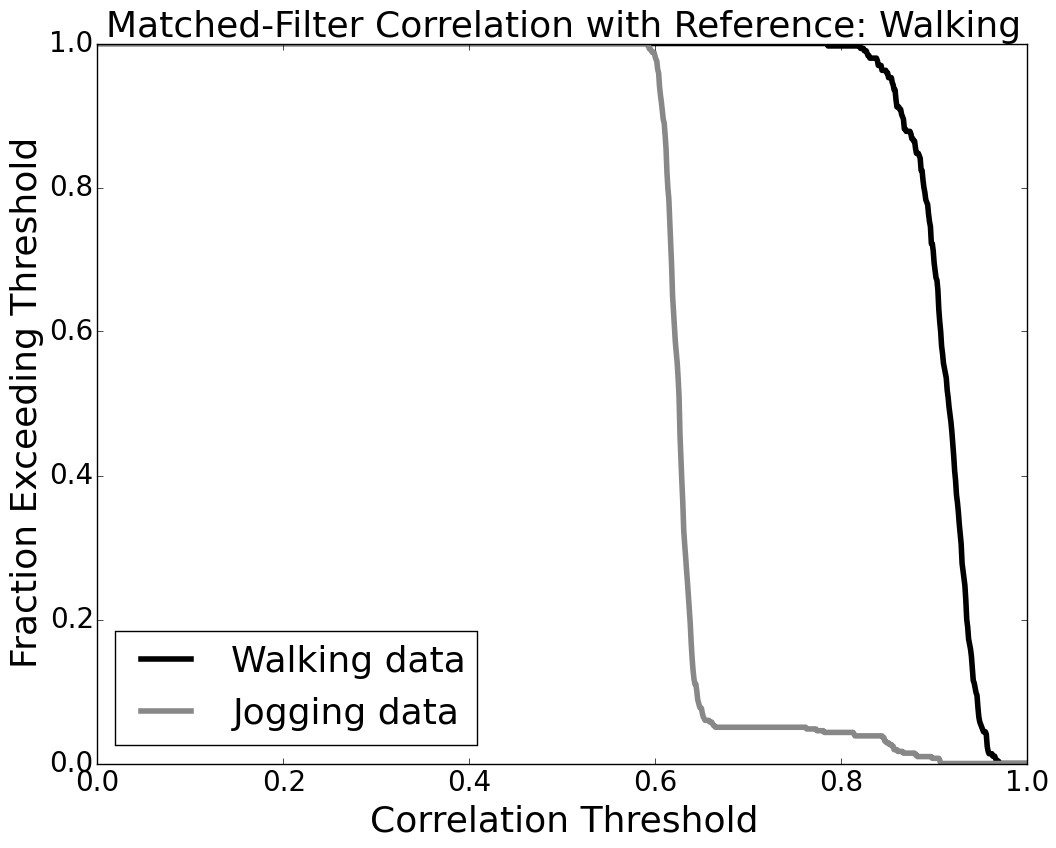
\includegraphics[width=0.45\textwidth]{fraction_threshold_walking_to_jogging.png}}
  \quad
  \subfloat[\label{fig:frac_walking_bicycling}]{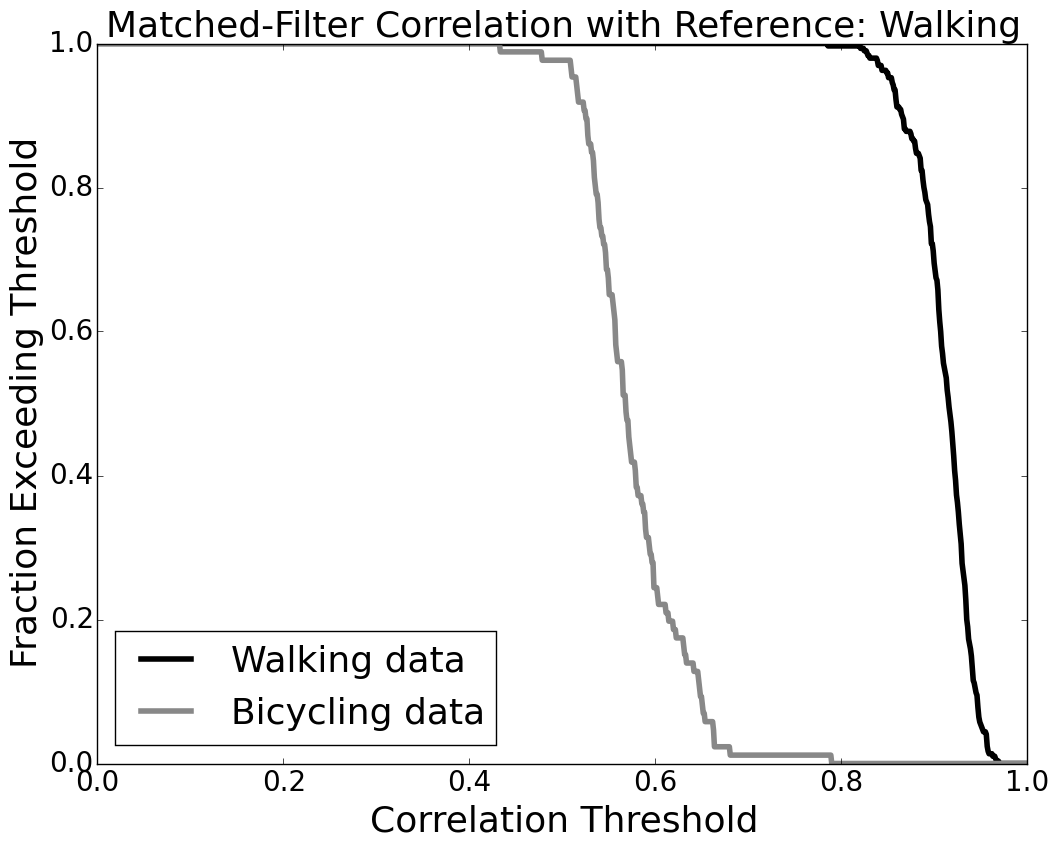
\includegraphics[width=0.45\textwidth]{fraction_threshold_walking_to_bicycling.png}}
  \centering
  \quad
  \subfloat[\label{fig:roc_walking_jogging}]{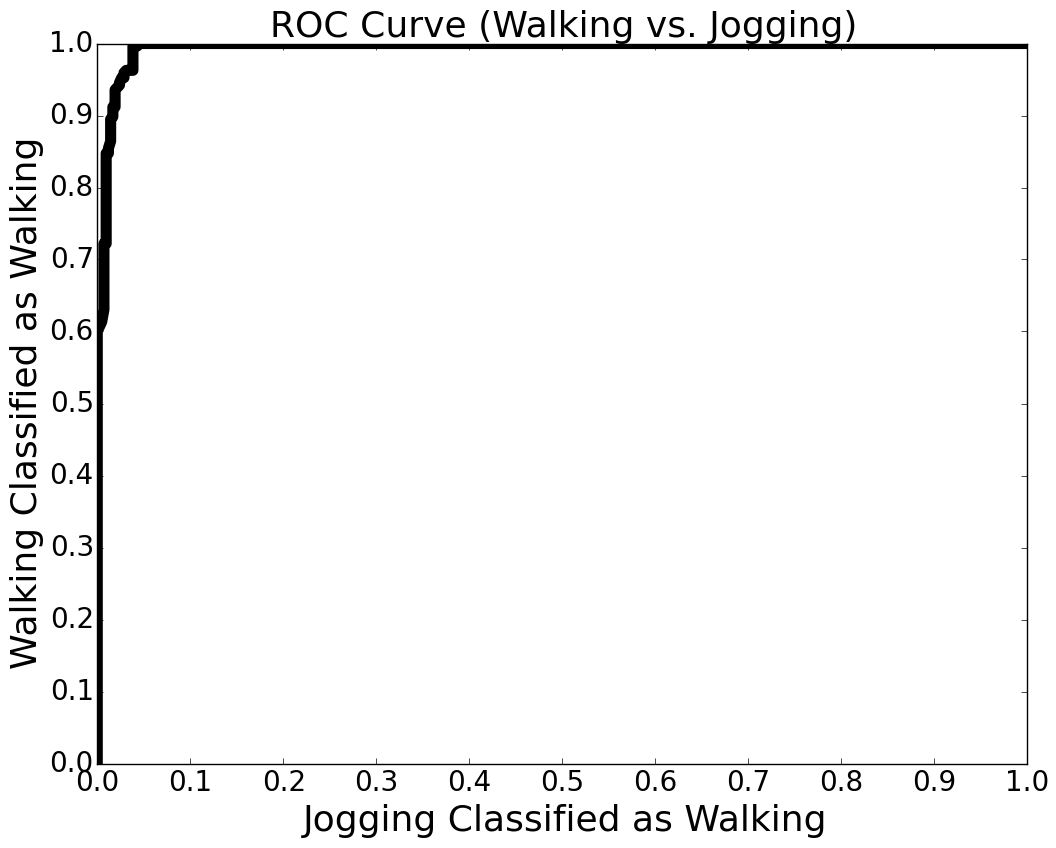
\includegraphics[width=.45\textwidth]{ROC_walk_to_run.png}}
  \centering
  \quad
  \subfloat[\label{fig:roc_walking_bicycling}]{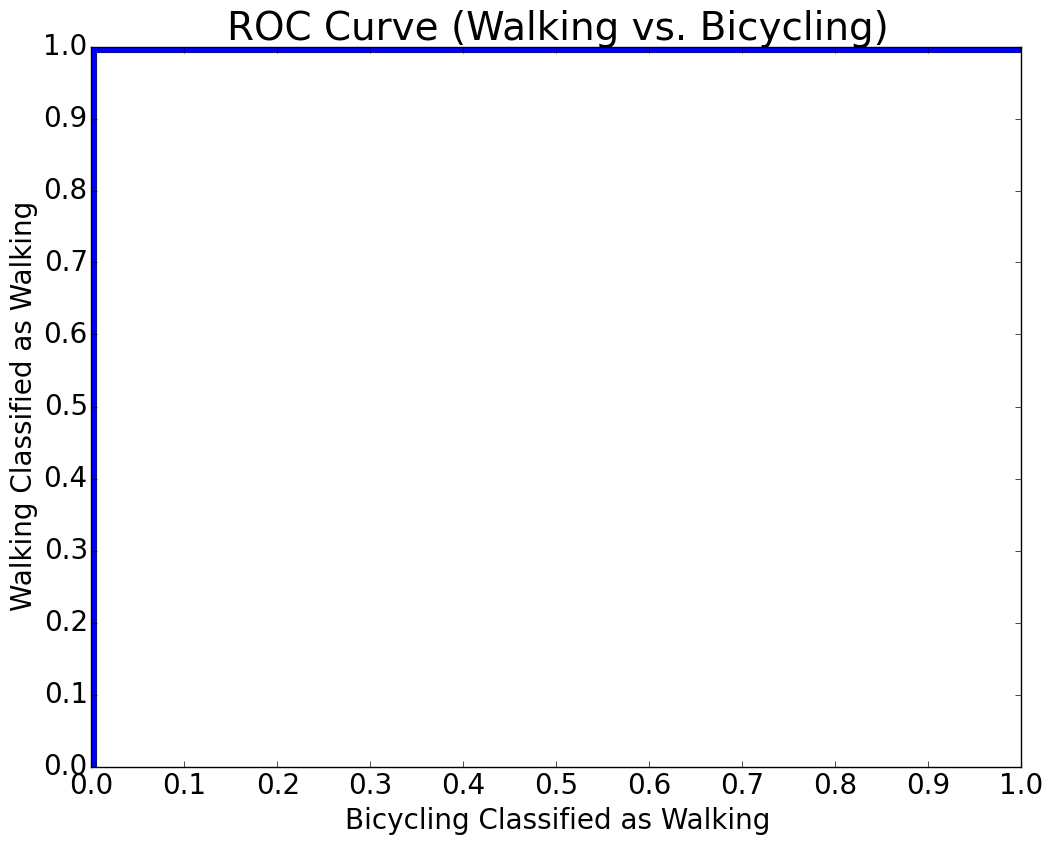
\includegraphics[width=.45\textwidth]{ROC_walk_to_bike.png}}
  \caption{Matched-filter performance comparing jogging and bicycling data against a reference for walking. Results produced at decimation 8. Figures (c) and (d) are the corresponding ROC curves produced from (a) and (b) respectivley.}
  \label{fig:MF_performance}
\end{figure}
%
Figures \ref{fig:frac_walking_jogging} and \ref{fig:frac_walking_bicycling} show the fraction of the correlation results that exceed the given correlation threshold when comparing the walking data reference to the given activity.
As we would expect, walking data matches better to walking data than the other activities.
ROC curves were produced from these corresponding results in \subref{fig:roc_walking_jogging} and \subref{fig:roc_walking_bicycling} to illustrate the effectiveness of the matched-filter as a classifier.
Figure \ref{fig:MF_performance} shows the comparison to bicycling.
Because the bicycling motions are considerably different from walking relative to jogging, we would expect better performance from bicycling.
%
%\FloatBarrier
%
\subsection{Throughput Performance}
%
To assess the real-time processing potential of the algorithms outlined in this paper, a throughput assessment was performed on the MSP432P401R microcontroller with varying parameters.
The Texas Instruments - MSP432P401R is a low power plus performance microcontroller that is based on the ARM 32-Bit Cortex-M4F processor.
Some of the notable features of the MSP432P410R is having a clock frequency of 48 MHz, 64 kB SRAM, 256 kB Flash Memory, and has an IEEE 754-compliant single-precision Floating-Point Unit (FPU) and Memory Protection Unit (MPU).
The single-precision processing capability on this unit provides us with a sufficiently large dynamic range necessary to process the algorithms that fixed-point processing cannot provide.
The 64 kB of SRAM provides sufficient space to process the results found in figure \ref{fig:timing} and
the 256 kB is more than enough flash memory to store the program and data references.
The clock frequency operates at 48 MHz which determines the execution speed.

\begin{figure}[!ht]
   \centering
   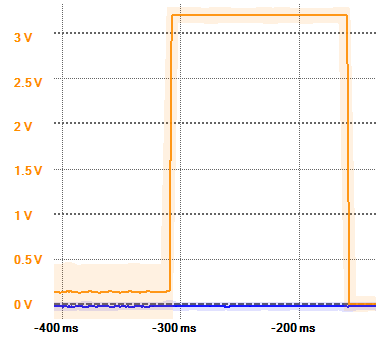
\includegraphics[width=0.45\textwidth]{32Hz_4sec_8downsample_2Reference_Pulse.PNG}
   \caption{Oscilloscope output used for measuring the processing time of the algorithms on the MSP432. This is a case setup of 32Hz sampling frequency over a 4 second time window with 2 references at decimation 8 showing the voltage output over time. Execution time is measured from the start to end of the ``high'' (3.3 Volts) time interval.}
   \label{fig:time_measure}
\end{figure}
%
The ``Analog Discovery 100MSPS USB Oscilloscope and Logic Analyzer'' oscilloscope was used for measuring the timing of the algorithms on the microcontroller.
When testing the execution speed, one of the General-Purpose Input/Output (GPIO) pins was connected to a Light-emitted diode (LED) that activates at 3.3 Volts (set high).
This is activated immediately before the beginning of decimation (start of algorithm processing) and deactivated immediately at the end of the matched-filtering (end of algorithm processing).
The execution time is then recorded on the oscilloscope to determine how long the GPIO was set high.
An example can be seen in Figure \ref{fig:time_measure}.

\begin{figure}[!ht]
   \centering
   \subfloat[\label{fig:multiple_comparison}]{\includegraphics[width=0.45\textwidth]{more_time_plots.png}}
   \quad
   \subfloat[\label{fig:timing_refs}]{\includegraphics[width=0.45\textwidth]{one_and_two_references.png}}
   \caption{Timing results with varying sampling frequencies, time-window lengths, and number of references used for the matched-filter on the MSP432 microcontroller processor. The time window used for (b) is 4.0 seconds.}
   \label{fig:timing}
\end{figure}
%
Randomized data was used for the purpose of analysing the throughput performance on the device while varying the parameters.
Figure \ref{fig:multiple_comparison} shows the execution time with varying time-window lengths and sampling frequencies while maintaining two references used in the matched-filter process while operating at decimation $2$.
Because the FFT dominates the processing load, and was optimized for even powered factors, one can observe better throughput at radix 2 valued time-window lengths and sampling frequencies followed by other even valued time lengths and sampling frequencies. Both $62$Hz and $50$Hz have only one factor of $2$ hence the expectation that a sampling frequency of $62$Hz processing time is longer than the $50$Hz.
Figure \ref{fig:timing_refs} shows the execution time over a $4.0$ second time window at decimation $8$ while varying the sampling frequency and number of references. Because the pre-processing execution time does not change with the number of references, it's observed that matched-filtering accounts for roughly $80$\% of the processing while pre-processing accounts for the other $20$\% when processing for a single reference.
%
\section{Conclusion}
Matched-filtering algorithms can be used for activity classification.
They can also be performed in real-time on a microcontroller such as the MSP432.
The algorithms consist of a training module in which the device is trained to identify the user’s activity along with a real-time activity classification module which uses the stored references that are produced by the training module in order to actively classify a user’s activity.
Although the matched-filtering algorithms require significant processing power, the data undergoes dimensionality reduction and decimation in order to reduce the required computational resources prior to being analyzed.
The algorithms were validated by using the Kinetisense accelerometer sensor to collect walking, jogging, and bicycling data.
The training module was ran on the data to produce references of the activities.
The data was compared to the walking reference and it was shown that the walking data matched well with the walking reference while the jogging and bicycling data did not match as well.
The algorithms were also executed on the MSP432.
Since FFT calculations dominate the processing time and work best with data that has radix 2 number of points, timing tests results demonstrate that radix 2 time-window lengths and frequency values result in faster processing times.
%
\appendices
%
\ifCLASSOPTIONcaptionsoff
  \newpage
\fi
%
\bibliographystyle{plain}
\bibliography{reference}
\end{document}
